

\documentclass[11pt]{article}
\setlength{\topmargin}{-.5in}
\setlength{\textheight}{9in}
\setlength{\oddsidemargin}{.125in}
\setlength{\textwidth}{6.25in}

 \usepackage{graphicx}
 \graphicspath{{images/}}
\begin{document}

\title{A User Model in Search for People with Autism}
\author{Esha Massand\\
MSc Computer Science Project Proposal\footnote{This proposal is substantially the result of my own work, expressed in my own words, except where explicitly indicated in the text. I give my permission for it to be submitted to the JISC Plagiarism Detection Service. }}
\date{\today}
\maketitle


\begin{abstract}
The current proposal presents my objective to research and build a user model within Search, to address the downfalls of current Search tools for individuals with Autism Spectrum Disorder (ASD). The user model will be built around the core features of ASD. The model will be applied to results returned from a synthesis of three leading existing search engines. The final product will be integrated with motion controllers, with the aim to enhance the user experience and the interface of Search for people with ASD.
\end{abstract}

\tableofcontents

\section{Introduction}
\subsection{Problem Statement} \label{problem}
Most search engines apply a general user model to refine search queries. The user models apply algorithms and weightings to each parameter, e.g., auto-complete, query understanding, site and page quality signals, user content and synonym snippets. No research to date has examined the experience of user search for individuals with Autism Spectrum Disorder (ASD), and whether these user models need to be adjusted for this subgroup. Although people with ASD are relatively proficient with technologies, we argue that the user models that underlie the way in which search queries are handled are different, and the needs of the user differ to the mainstream models. This project aims to build a suitable user model of ASD to address this gap.
As it has been shown that individuals with ASD are more engaged (show sustained attention) when using technology that is receptive (games, responsive consoles, motion controlled devices) and interactive compared to technology that is not, this project will combine interactive, Motion Recognition hardware with Search to improve the User Interface and architecture of Search for individuals with ASD.

\subsection{The Role of Context In Search}
It is unlikely that any given page on the web will contain a word or phrase that means exactly (or nearly) the same as another word or phrase in that language (e.g., shut and close). How is it then that your search engine of choice picks these phrases to mean the same thing, and returns them synonymously in the results of your query? Well, quite simply put, it is by virtue of the fact that each of their neighbouring words and associations are similar. These are indirect, higher-order associations, and provide the context in which the search engine can index keywords. This context plays a crucial role in search; first, in the interpretation of the query put forward by the user, and second, the context is reflected in the results returned to the user.

\subsection{What is ASD?}
The prevalence of Autism Spectrum Disorder (ASD) is amongst the most common neurodevelopmental condition and it is currently estimated that 1/68 children meet criteria for ASD (CDC, 2014). ASD is five times more common amongst boys than girls (1/42 boys, and 1/189 girls). According to the DSM-V (2013) diagnostic manual, ASD is characterized by persistent and early deficits in reciprocal social interaction and repetitive behaviours. Individuals vary from high functioning to low functioning (along a spectrum), with behaviours emerge around 2 or 3 years of age. 

\begin{center}
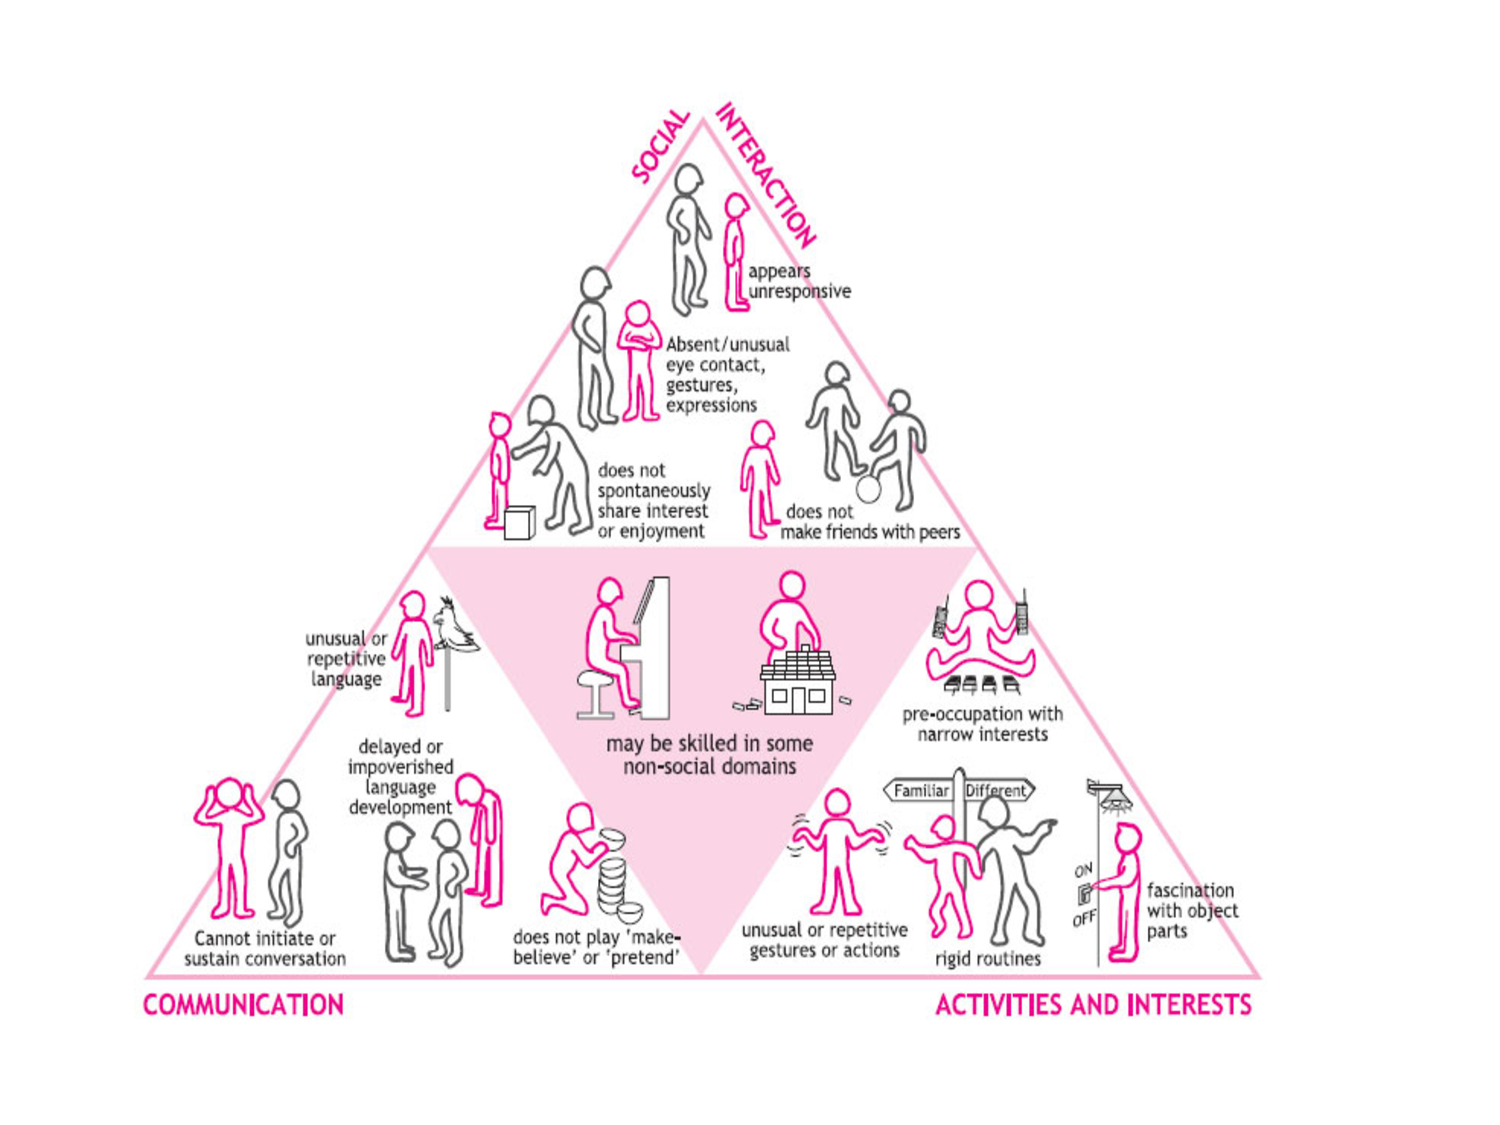
\includegraphics[scale=0.5]{asd}\\
The ASD Triad (source: http://media.kingdown.wilts.sch.uk/mod/page/view.php?id=7374)
\end{center}

\subsection{The Problem: Current Search Tools for people with ASD} \label{problem}
Search engines assume that the user is context-driven, and they attempt to model the user's intent using higher-order contextual information gathered from available web pages. This process also models the human brain's ability to extract context and semantic associations from information. However, what if the user was context-insensitive\footnote{Or, less context-sensitive}  and preferred a detail-focused processing style? They would intuitively form search queries very differently. For example, individuals with ASD are less likely to engage in a relational (hierarchically organized) style of processing (Bowler et al., 2009) suggesting that relating information in a hierarchically organised framework is less likely. Hierarchical organisation implies a great deal of flexibility and mental-shifting, as a simple example, in a search for 'apple', it would imply awareness that the word is related to 'pear' but also to 'fruit'. Awareness of this latter relation also suggests awareness that 'apple' is related to 'pomegranate'. Of course, in genuine search queries these associations can get very complex very quickly. Generally speaking, individuals with ASD prefer, and are more likely to engage in an item-specific processing style, and, whilst intelligent cognition is definitely possible, search queries are more likely formed of first-order associations\footnote{Of course there is a great deal of individual variability in Autism Spectrum Disorder.}. \\
\\Several Psychology learning and intervention studies for individuals with high functioning ASD have suggested that assimilation and accommodation of new information is most appropriate when:\\
\begin{enumerate}
\item Information is concrete (not abstract).\\
\item Information is presented in small manageable chunks.\\
\item Information is not verbally ?overloaded? (not too many words).\\
\item Information is presented in the expected way and does not deviate from this.\\
\end{enumerate}
Several interventions have been built around this body of literature (www.autismspeaks.org).\\
Given these findings from the literature we can make several adjustments to current Search tools to enhance their benefit for people with ASD. For example, a user with ASD would 
have improved user-experience if their search results:\\
\begin{enumerate}
\item Were assessed (before presentation to the user) for the Key Word In a suitable Context.\\
\item Followed a similar order of semantic association, in line with the search query itself. \\
\item Were smaller and more manageable.\\
\item Were visually consistent.\\
\item Had a high degree of verbal consistency/similarity with the search query.\\
\end{enumerate}

\subsection{Proposal Organisation}

This proposal outlines my research to date on the field of Search, ASD, and User Interfaces. I also include my preliminary planning of the methods I will use to implement the enhanced Search tool for ASD. The remaining chapters discuss:
\begin{enumerate}
\item in Section~\ref{What should Search offer people with ASD}, I give a brief introduction to Search engines, and the downfalls of current Search engines for individuals with ASD. I discuss the motivation behind the proposed work
\item in Section~\ref{Existing Combination/Advanced Search Engines}, I will discuss the existing combination/advanced search engines
\item in Section~\ref{}, I briefly discuss API's and Libraries that I will use during the project, including Custom Search Engine APIs such as the Google Custom Search API, and Yahoo BOSS, Lucene Key Word In Context
\item in Section~\ref{}, I discuss the potential for user modeling within Search
\end{enumerate}



\section{What should Search offer people with ASD?}\label{What should Search offer people with ASD}
\subsection{Search and Learning}
The Internet is one of the largest resources of information, and can be searched by users from different areas of the world relatively quickly. Search engines allow users to collate hundreds of links on a single topic, using only a few words or phrases. The variety of information returned is vast, and the depth of users’ searches can be determined by more advanced refinement options \footnote{For example, using the keyword NOT, or, by applying precedence to a selection of search query terms likely to be returned. This implies the user has some understanding of the keywords likely to be picked up and returned by the search engine. With this knowledge the user may choose to do a targeted search for just some specific key term.} . Search is an important learning tool; its significance is duly noted because of the learning benefits it brings for children and adolescents as they begin to navigate the Internet and gain an understanding of several subjects. 
Typically developing children are taught how to navigate search engines in school from a very young age (Google, Yahoo, Bing and other search engines), although other child-friendly searches exist (e.g., Ask Kids or KidRex). These child-friendly search engines’ aesthetics are designed specifically for children. They also prioritise the users ‘online safety’; in other words the results of the search have been filtered to include age-appropriate material, and they are visually presented in a more stimulating way for children.  Individuals with ASD represent a subset of the population who are not as engaged by interfaces of current search engines, like Google, Yahoo and bing, so they lose out on this important way to learn new information. The aim of the system is to be tailored to the needs of individuals with ASD, so that they do not lose out on this important learning tool.

\subsection{Clues from virtual reality and gaming}
Almost all teenagers (97\% of those aged 12-17) use a computer, web, portable or console devices, 73\% of which is desktop or laptop based. Teenagers with ASD also use technology and spend a substantial amount of their time using devices \cite{Shane and Albert}. They are proficient, and use these devices with relative ease, showing high levels of engagement with consoles like the Xbox (Kinect) or Wii, Portable Gaming Devices (Nintendo DS), or cell phone or handheld device. For individuals with ASD, computer-based technologies can provide a stable, consistent learning environment that can be customized (Moore, McGrath \& Thorpe, 2000). The proposed system will utilize motion controllers (used by the Wii, Kinect) to facilitate engagement with Search. 

\subsection{Motion Controllers}
Motion recognition devices can be programmed to make consistent responses to environmental triggers. This is unlike real-world situations where environmental responses are not always consistent and may require further interpretation or ‘guess-work’. These controlled and interactive environments have shown promise for improving social communication skills and reducing repetitive behaviours (Games for Health, 2012).

\subsection{Visual not text-based}
People with ASD may prefer a more visually-oriented approach to search – one that doesn’t require sustaining a search query in working memory / attention and abstracting a question, to type it into a white box on a screen. It is likely that search can be just as powerful for learning and stimulating for them, if within an appropriate user interface that caters for these individuals needs.


\section {Creating a User Model of ASD}
\subsection{What is a user model?}
A user model is a collection of information associated with a particular user, with which a system can adapt its behavior in order to customize in line with the user’s needs. The concept of user modeling has strong implications for the way in which humans and computers interact; by creating a representation of the user, the system can be better informed about how to behave in various circumstances, for example, the system can acknowledge a specific kind of user’s needs, preferences, likes, dislikes, goals, plans, knowledge, and skill. The system can maintain this knowledge whilst interacting and adapting its behavior with the user.
Persona development will support the user modeling process by identifying particular characteristics of individuals with ASD in Search. An individual’s personal information pertaining to the persona, will be stored in a user profile which will contain information such as age, gender, lifestyle, frequent tasks, tools used, resources commonly used and crucially for this project, the profile will include information about diagnosis (Autism, Asperger, language ability).

\subsection{Types of user models}
User models can be static, and unchanging (i.e., no algorithms are used in order to teach the model about the changing preferences of the user, and no new information is fed into the model), or dynamic (representation of the user with their up-to-date changes in interests, and recent interactions with the system). Alternatively, user models can be stereotype
This means they utilize demographic information to classify users into distinct subtypes. The system infers or assumes other characteristics about this subset of users by making use of data gathered from other users also included within this subset. Lastly a user model can be highly adaptive and try to model the one user on their own, without stereotyping or inferring the characteristics of the user. This type of user modeling requires a large amount of data collection prior to its implementation.
\\The model can gather information through direct interaction with its user (e.g., via a registration process), by observing and interpreting the users actions, or, by a combination of both, that is, the system may ask for feedback, and alter its approach depending on the user’s behavior.

\subsection{Benefits and difficulties of user modeling in Search}
The model needs to collect data before it can predict the user’s needs with accuracy, but once this is achieved, information can be presented according to the user’s knowledge, ability and goals. It can also effectively filter out irrelevant information and rank the remaining search results in the most relevant way according for the user.
Creating a user model is not an easy task. The designer of the system has to set the weights of the parameters for the information that is fed into the model, and decide what course of action to take when two pieces of information may conflict. Some of the difficulties associated with deciding the priorities of elements of the model will be dealt with in a feasibility test (section X), and be refined with user-feedback /testing. Other elements of the user model will be based on modeling well-researched cognitive processes in ASD (for example, a user model that focuses on first-order, or, item-specific relations to form a search query, rather than hierarchical relations to form a search query).  

\subsection{Adaptive / Personalised Search}
Adaptive or Personalised search, is one way in which search engines including Google, Yahoo and Bing have attempted to tailor the search results for their users. The feature was first introduced as part of a GoogleLabs project in 2004 and implemented in 2005. It associates each user search with a HTTP cookie – this is a piece of data (a text file) sent from the website and saved in the users’ browser when the user navigates that website. These cookies contain information such as login information (gender, age), preferences (languages, interests) and other information about previous searches based on site traffic. The cookies allow the website to ‘remember’ stateful information about what buttons the user clicked on, or what sites they visited. This cookie record allows the search engine to return results that are highly relevant to the search query, but also highly relevant to the pages that the user visited through previous searches. When personalised or adaptive search is combined with GPS data from a smartphone or device, it can provide useful information about the places that user has previously visited to higher rank local items in the users returned results. This creates a personalized or adaptive web search, as the feature allows the web search to be tailored to the user’s preferences over the course of time, and as more searches are recorded.

\subsection{Disadvantages of adaptive search for individuals with ASD}
Although adaptive search seems to have significant user benefit in terms of relevance to the user for that search query, it decreases the likelihood that the user encounters new information and biases the results towards the users location and their previous site traffic.  This has the unwanted effect of creating a filter bubble (Pariser, 2011), which is argued to close us off from important and relevant information and create a personal ecosystem of information for one particular user, creating the impression that “our narrow self interest is all that exists”. The filter bubble also has potential privacy problems, as the user may be unaware that the search has been specifically tailored towards their interests and they wonder why things that they have previously searched for have become more and more relevant. The filter bubble may positively reinforce restricted interests in ASD as the user constantly receives feedback about their previous (idiosyncratic and personalized) searches without being able to break out of that repetitive loop. 
Recent research has suggested personalization also increases ‘background noise’ relative to the search results (Briggs, 2014). Briggs (2014) also suggests that there is a carry-over effect in personalized search for the users, whereby prior search results influence the results of subsequent searches \footnote{It should be noted that personalization of search results generally takes a lower priority for the ranking algorithms than the URLs ranked top in terms of their relevance for the search query.}.  Nevertheless this carry-over may be disadvantageous for people with ASD as it muddies their search space with previous interests, and provides unwanted distraction from the task at hand. 
It appears that in order to produce a search tool specifically tailored to reduce the filter bubble effect in ASD, widen the information gateway and reduce the possibility for restricted and repetitive searches, what is needed is a reprioritization of the weighting on previous search results in adaptive/personalized searches, in order to focus users on the current search at hand and limit the possibility that users get trapped in a spiraling loop of ever-narrowing user-relevant information and over personalization of self-reinforced information ecosystems.

\subsection{Where will the User Information be Stored?}

\section{Existing Combination/Advanced Search Engines}\label{Existing Combination/Advanced Search Engines}
No question about it, Google is still the world’s most popular search engine, and remains the most used search engine in the world (http://searchengineland.com/google-worlds-most-popular-search-engine-148089, 2013).  However, other highly capable search engines are being offered as alternatives, for example the Bing search engine offered by Microsoft, Yahoo, Ask, to name a few, and they deserve some exploration (http://www.makeuseof.com/tag/4-search-engines-that-combine-google-bing/).

\subsection{Bing vs Google}
\begin{center}
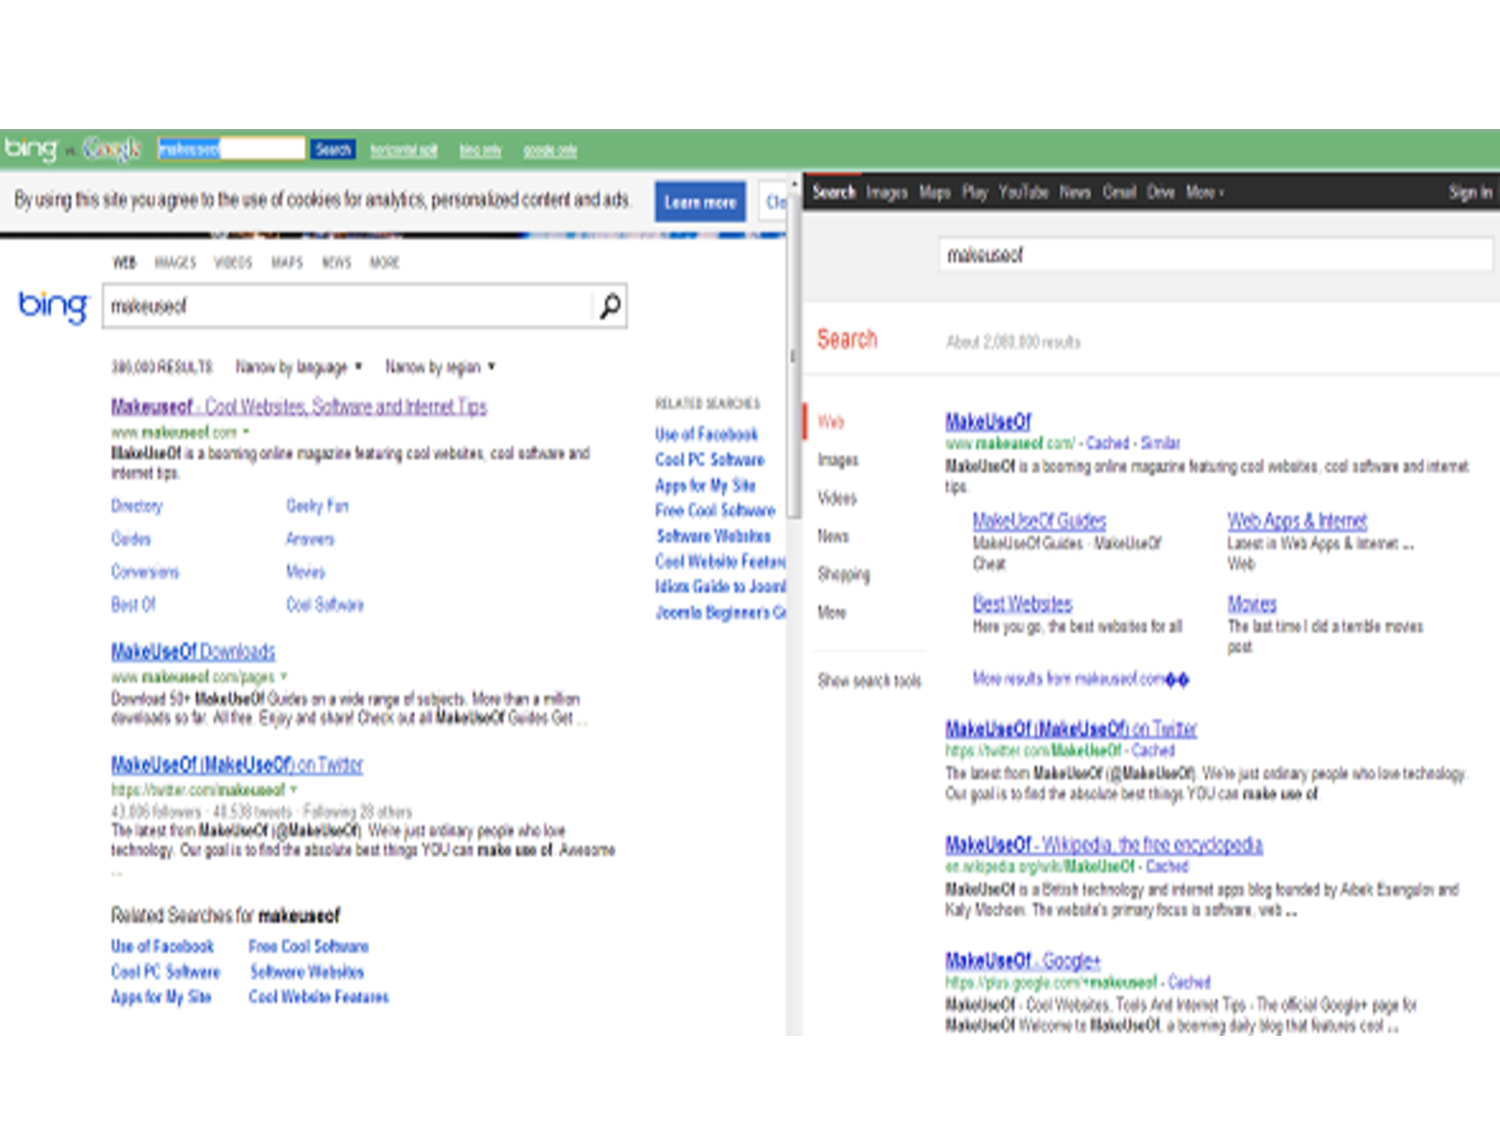
\includegraphics[scale =0.5]{bingG2}\\
\end{center}
Bing vs. Google presents the users’ search query results from both search engines to allow the user to make a comparison (the Google and Bing results can be presented vertically or horizontally beside each other), and provides the experience of navigating both search pages simultaneously.  The number of other personal preferences options is very limited (the orientation of the results is just about all the user has the option to choose).

\subsection{Qrobe.it}
Qrobe combines three search engines’ results (Google, Bing and Ask) and presents them conveniently on one page. Unlike Bing vs
Google the user can search ‘web’, ‘images’ or ‘popular’ to reveal stories from Reddit. Qrobe.it also has a ‘cheatsheet’ that allows user to search using shortcuts, which may prove useful to a seasoned Qrobe user. Qrobe unfortunately has no API for developers to use to extend its functionality further.

\subsection{AskBoth}
AskBoth – is a work in progress, and combines both Google and Bing, with a section in the middle dedicated to twitter , just like Bing vs. Google but AskBoth argues that the selling points for the site are it’s ‘uncomplicatedness’, aesthetics and user experience – which promises to be particularly good (that is, has promised, since 2009!).

\subsection{Spectra}
Spectra takes searching from Google, Bing and Yahoo engines one-small-step-further. This site allows users to assign weights and determine the way results are displayed. Spectra gathers the search results, ranks them and displays them according to their algorithm. 

\subsection{Conclusions and ways forward}
All these search engines allow users to see more results than what one search engine alone would present, they often do this with a cost -- redundancy. The benefits are that there is more information presented to the users at once but often at a cost of ‘cognitive overload’ and/ or near –duplicates. This is not ideal for users with ASD, as this is precisely the opposite of what the systems aims and objectives were see Section ~\ref{problem}.
To date, a user model for ASD within Search has not been built. The following section presents the proposed system that will try and address this issue.


\section{Proposed Search Page and Controller Web Application}

Insert Image Here!!!!\\The project will produce a search engine designed to enhance the user experience within search for people with ASD. Below I list the core and non-core features to include:


\section{Core Features}
\begin{enumerate}
\item A synthesis of the results from three of the largest and most popular search engines (Google, 67.5\%, Microsoft Bing 18.4\% and Yahoo 10.3\%) (Adam, 2014)

\item Creating a user model to apply to these results to filter them according to specific user needs. The model will be XXXX

\item A redefinition of the returned results using history logs: search result relevance/ranking will reflect the abstractness of the user query, refining results to return pages not just highest overlap of key terms, but doing contextual analyses within those results rank those pages depending on words in context. Possibly ranking a page with a number of pictures / picture tags higher than those with many words. 

\item Using motion controllers to enhance embodiment within search, and enhance the search query process. One idea is to have users be able to physically 'grab' results, to save them to inspect later. This will mean they do not have to 'track' or remember their navigation around search, but rather, filter their own results at an earlier time point. I will investigate the use of the LEAP motion controller, the Oculus Rift, Xbox as possible avenues for devices.

\item Get user feedback by testing the web search with the LEAP motion controller, with a group of individuals diagnosed with ASD.

\item Revise the model and the ideas to choose the best possible approach/tools to tackle search (experience) optimization for people with ASD.

\end{enumerate}

\section{Non-core Features}
\begin{enumerate}
\item Changing the user interface. This includes many visual changes, for example, colours and contrast, and other personalisable aesthetic changes.

\item	I will include a variation on the ‘type’ of search using the threeJs framework – I will build a search that completely presents ‘YouTube’ videos, with no text on the page if the user prefers to understand more about whether users would prefer their results returned to them in the form of YouTube videos.

\item	User testing and feedback with other motion controller devices, possibly the Oculus VR Rift, Xbox Kinnect.

\end{enumerate}
I hope these findings will provide novel insights into the needs and wants of individuals with ASD within search, and enable future development and interventions within these information streams and communication channels. Ultimately, I want to build a user-oriented search system, so that individuals with ASD do not have to 'fit in', but rather benefit from them.

\section{Implementation of the System}\label{implementation}
\subsection{Selection of Search Engines}
The three most popular search engines (as calculated using an average of the unique monthly visitors) are Google (1,100,000,000 estimated monthly visitors), Bing (350.000.000 estimated monthly visitors) and Yahoo! (300,000,000 estimated monthly visitors) (www.eBizMBA.com; 2015). Google is the most recent and goliath question-answering system (query volume = 64.5\% Lella, 2015), and the word has become synonymous with the word ‘search’ on the web. This search engine is often considered the most innovative and dynamic, and is the most popular amongst users worldwide (using global traffic rank figures, in March 2015). Yahoo (2003) was the first ever web directory service; it has stronger advertising and e-commerce partnerships and has a query volume of 19.8\%. Bing (Microsoft’s answer to search, previously known as msn search), was officially launched in 2005, and has a query volume of 12.8\%, which is substantially less than Google, but nevertheless, is within the top 3 search engines. Other search engines include Ask, AOL, WOW, which will not be included in the search system proposed here in order to limit the redundancy of the search results (of which there will already be a fair amount). 

\subsection{APIs, Text-Search Libraries }
I will be using API’s to work with the three search engines outlined in the above section. Although the same information could be gathered by inspecting the source code for the pages that return the search query results, the API’s were considered to be far more efficient in doing so. 

\subsubsection{Google Custom Search}
Google Custom Search (GCS) allows the creation of a search engine that can be configured to search web pages and images. It is highly personalisable and comes with an API that supports the development of a custom search engine project on a pay per search basis. Once signed up, the GCS requires a consumer key and secret, which are hardcoded in the development of the search.
The API has methods which allow the user to …\\
However, this API needs to be used in conjunction with a textual-search library in order to reach the Goals of this project (the API does not offer Key Word In Context Search in order to trace the contextual information being returned to the user). Costs \$0.01/search.

\subsubsection{Yahoo BOSS}
Just like Google Custom Search, the Yahoo BOSS API required the creation of a search engine project (pay per search) with a consumer key and secret. The API is also easy to use and offers the same functionality as the CSC but again is not sufficient alone to reach the goals of the project. Costs \$0.01/search.

\subsubsection{Bing Search API (Data)}
The Bing Search API, similar to Yahoo BOSS and GCS will produce results for Web, Images, News, Videos, Related Search. Bing Search API also includes spelling suggestions based on the query entered. Costs \$0.00/search (max 5000 searches/month)

\subsubsection{Faroo API}
Is a free alternative API to Google Custom Search API (business), Yahoo BOSS API  (commercial) and Bing Web Search Enterprise (commercial). It offers the possibility to do aWeb Search, with more that 2 billion pages indexed by Faroo. In addition to English, German and Chinese results can be returned, sorted by relevancy.  Faroo can return news search (articles from newspapers, magazines and blogs) and sort results by publishing date, with author and article image. Trending news pages are also indexed and can be grouped by topic. Topics sorted by buzz (number of sources reporting on same topic). Faroo also offers suggestions with auto-completes for misspelled items in the search query \cite{faroo}.

\subsubsection{Apache Lucene Library}

\subsubsection{Google+ API}





\begin{thebibliography}{100}

\bibitem {games} Games for Health, 2012 Screen-based technologies and Autism. 1: 248-53


\bibitem {briggs}Briggs, Justin. A Better Understanding of Personalized Search. Retrieved21 April 2014.


\bibitem {Brusilovsky}Brusilovsky, P. and Tasso, C. (2004) User modeling for Web information retrieval. User Modeling and User Adapted Interaction 14 (2-3), 147-157.


\bibitem {CDC}Developmental Disabilities Monitoring Network Surveillance Year 2010 Principal Investigators; Centers for Disease Control and Prevention (CDC). Prevalence of autism spectrum disorders: Autism and Developmental Disabilities Monitoring Network, United States, 2006. MMWR Surveill Summ.2009; 58(10):1–20


\bibitem {Shane and Albert}J Autism Dev Disord. 2008 Sep;38(8):1499-508. doi: 10.1007/s10803-007-0527-5. Epub 2008 Feb 22.
Electronic screen media for persons with autism spectrum disorders: results of a survey.
Shane HC1, Albert PD.


\bibitem {Lasater}Lasater, M. W., \& Brady, M. P. (1995). Effects of video self-modeling and feedback on task fluency: A home-based intervention. Education and treatment of children, 18, 389-407.


\bibitem {Pariser}Eli Pariser (2011) First Monday: What's on tap this month on TV and in movies and books: The Filter Bubble by Eli Pariser". USA Today. 2011. Retrieved April 20, 2011. Pariser explains that feeding us only what is familiar and comfortable to us closes us off to new ideas, subjects and important information.


\bibitem {Economist} Invisible sieve: Hidden, specially for you. The Economist. 30 June 2011. Retrieved June 27, 2011. Mr Pariser’s book provides a survey of the internet’s evolution towards personalisation, examines how presenting information alters the way in which it is perceived and concludes with prescriptions for bursting the filter bubble that surrounds each user.

\bibitem {MacDuff} MacDuff, Krantz, \& McClannahan (2001). Prompts and prompt-fading strategies for people with autism. In C. Maurice, \& G. Green (Eds.), Making a difference: Behavioral intervention for autism (pp. 37-50). Austin, TX: Pro-Ed.


\bibitem {Sherer}Sherer, M., Pierce, K. L., Paredes, S., Kisacky, K. L., Ingersoll, B., Schriebman, L. (2001). Enhancing conversation skills in children with autism via video technology. Behavior Modification, 25, 140-158.


\bibitem {Thiemann}Thiemann, K. S., \& Goldstein, H. (2001). Social stories, written text cues, and video feedback: Effects on social communication of children with autism. Journal of Applied Behavior Analysis, 34, 425-446.


\bibitem {Combining}Combining Search Engines: Existing Solutions Review
http://www.makeuseof.com/tag/4-search-engines-that-combine-google-bing/


\bibitem {Google}Google Remains the most popular search engine http://searchengineland.com/google-worlds-most-popular-search-engine-148089, (2013).  


\bibitem {Vaishnavi1}Sandeep Vaishnavi1 , Jesse Calhou , and Anjan Chatterjee (2001). Binding Personal and Peripersonal Space: Evidence from Tactile Extinction. Journal of Cognitive Neuroscience 13:2, pp. 181–189


\bibitem {Lella}Lella, Adam (2014-04-15). comScore Releases March 2014 U.S. Search Engine Rankings. ComScore.com. Retrieved 2015-02-21



\bibitem {googlebing} http://www.makeuseof.com/tag/4-search-engines-that-combine-google-bing/


\bibitem{faroo}http://www.faroo.com/hp/api/api.html\#description

\end{thebibliography}
\end{document}
